\documentclass[twoside,twocolumn]{article}

\usepackage{blindtext} % Package to generate dummy text throughout this template 
\usepackage{graphicx}
\usepackage[sc]{mathpazo} % Use the Palatino font
\usepackage[T1]{fontenc} % Use 8-bit encoding that has 256 glyphs
\linespread{1.05} % Line spacing - Palatino needs more space between lines
\usepackage{microtype} % Slightly tweak font spacing for aesthetics

\usepackage[english]{babel} % Language hyphenation and typographical rules

\usepackage[hmarginratio=1:1,top=32mm,columnsep=20pt]{geometry} % Document margins
\usepackage[hang, small,labelfont=bf,up,textfont=it,up]{caption} % Custom captions under/above floats in tables or figures
\usepackage{booktabs} % Horizontal rules in tables

\usepackage{lettrine} % The lettrine is the first enlarged letter at the beginning of the text

\usepackage{enumitem} % Customized lists
\setlist[itemize]{noitemsep} % Make itemize lists more compact

\usepackage{abstract} % Allows abstract customization
\renewcommand{\abstractnamefont}{\normalfont\bfseries} % Set the "Abstract" text to bold
\renewcommand{\abstracttextfont}{\normalfont\small\itshape} % Set the abstract itself to small italic text

\usepackage{titlesec} % Allows customization of titles
\renewcommand\thesection{\Roman{section}} % Roman numerals for the sections
\renewcommand\thesubsection{\roman{subsection}} % roman numerals for subsections
\titleformat{\section}[block]{\large\scshape\centering}{\thesection.}{1em}{} % Change the look of the section titles
\titleformat{\subsection}[block]{\large}{\thesubsection.}{1em}{} % Change the look of the section titles

\usepackage{fancyhdr} % Headers and footers
\pagestyle{fancy} % All pages have headers and footers
\fancyhead{} % Blank out the default header
\fancyfoot{} % Blank out the default footer
\fancyhead[C]{Patrones de Diseño $\bullet$ Octubre 2020 $\bullet$ } % Custom header text
\fancyfoot[RO,LE]{\thepage} % Custom footer text

\usepackage{titling} % Customizing the title section

\usepackage{hyperref} % For hyperlinks in the PDF

%----------------------------------------------------------------------------------------
%	TITLE SECTION
%----------------------------------------------------------------------------------------

\setlength{\droptitle}{-4\baselineskip} % Move the title up

\pretitle{\begin{center}\Huge\bfseries} % Article title formatting
\posttitle{\end{center}} % Article title closing formatting
\title{Patrones de Diseño} % Article title
\author{Yober Nain Catari Cabrera } 
\date{\today} % Leave empty to omit a date
\renewcommand{\maketitlehookd}{%
\begin{abstract}
	\begin{center}
		\textbf{Resumen}
	\end{center}
	Por más específico que un problema sea en el desarrollo de software, existe una gran probabilidad de que alguien haya enfrentado a un problema muy similar en el pasado, de cual en el momento se pueda modelar de la misma forma.\\
	La estructura de las clases se refieren al modelado, por lo que esta estructura conforma la solución de problema , que probablemente puede estar inventada. Si la manera de solucionar ese problema tiene los siguientes factores: extracción, explicación y reutilización en los múltiples ámbitos, se puede analizar que es un patrón de diseño de software.\\
	\begin{center}
		
		\textbf{Abstract}
	\end{center}
	No matter how specific a problem is in software development, there is a high probability that someone has faced a very similar problem in the past, which at the moment can be modeled in the same way.
	The structure of the classes refers to the modeling, so this structure makes up the problem solution, which can probably be invented. If the way to solve that problem has the following factors: extraction, explanation and reuse in the multiple domains, it can be analyzed that it is a software design pattern.
	\\
\end{abstract}
}

%----------------------------------------------------------------------------------------

\begin{document}

% Print the title
\maketitle

%----------------------------------------------------------------------------------------
%	ARTICLE CONTENTS
%----------------------------------------------------------------------------------------

\section{Introduccion}

\lettrine[nindent=0em,lines=3]{L}os patrones de diseño han demostrado ser un medio útil de
capturando soluciones de diseño probadas en el tiempo y facilitando su reutilización.
Los patrones apuntan a representar explícitamente el conocimiento de diseño que es
entendido implícitamente por profesionales calificados.
Quizás en ninguna parte el enfoque del patrón ha sido más efectivo
que en la ingeniería de software. Gamma y col. [1] describe el software
diseñar patrones como "descripciones de objetos comunicantes y
clases personalizadas para resolver problemas de diseño dentro de un
contexto particular ".
Las descripciones en la literatura de investigación a menudo colocan más
énfasis en características novedosas que en patrones de diseño recurrentes. Como un
resultado, puede ser difícil identificar, evaluar y volver a aplicar el diseño
en soluciones implementadas dentro de los marcos existentes


%------------------------------------------------
%-----------------------------------------------------------------
\section {Marco Teórico}\label{sec:3}
\subsection{Historia}
1965-1993: El término patrón fue debido al arquitecto Christopher Alexander en el año 1977, en su libro "A Pattern Language" define: "Cada patrón describe un problema que ocurre una y otra vez en nuestro entorno".

1994:Gang of Four publica el libro "Design Patterns: Elements of Reusable Object Oriented Software", conformada por Erich Gamma, Richard Helm, Ralph Johnson y John Vlissides. Lograron recopilar y recopilar una cantidad de 23 patrones de diseño que ahora son aplicados por expertos diseñadores de software orientado a objetos.

1996: Surge Java. La filosofía que llevaba esta era aprovechar el software ya existente. Facilitar la adaptacion del mismo a otros usos diferentes a los originales sin la necesidad de modificar el código ya existente.

2001: Se publica el libro, Patrones de arquitectura de aplicaciones de negocios. 

2003: Surge el Diseño Dirigido por Dominio tiene que ver con el diseño y la creacion de modelos altamente expresivos. Tambien crea modelos que esan comprensibles para todos los involucrados en el desarrollo de software.

Actualidad: Se aplican distintos patrones de diseño de acuerdo al modelo de negocio, una practica común es usar el modelo vista controlador como patrón de diseño base y usar partes o elementos de otros patrones de diseño que se ajusten a la solución.



\subsection{ Patrones de Diseño de Software}
Los patrones de diseño son soluciones típicas a problemas comunes en el diseño de software. Son como planos prefabricados que puede personalizar para resolver un problema de diseño recurrente en su código.
Un patrón de diseño es una descripción de clases y objetos comunicándose entre sí adaptada para resolver un problema de diseño general en un contexto particular.\cite{Tanembaum3}

\subsection{ Elementos de un patrón}
\begin{itemize}
	\item \textbf{Patrones de diseño creacionales:} nombre estándar del patrón por el cual será reconocido en la comunidad \cite{Tanembaum1}
	\item \textbf{Clasificación del patrón:} creacional, estructural o de comportamiento.\cite{Tanembaum1}
	\item \textbf{Intención:} ¿qué problema pretende resolver el patrón?\cite{Tanembaum1}
	\item \textbf{Motivación:} Escenario de ejemplo para la aplicación del patrón.\cite{Tanembaum1}
	\item \textbf{Consecuencias:} consecuencias positivas y negativas en el diseño derivadas de la aplicación del patrón\cite{Tanembaum1}	
\end{itemize}

\subsection{Clasificación de los patrones}
\begin{itemize}
	\item \textbf{Patrones de diseño creacionales}
	\\
	\\Son patrones de diseño que se ocupan de los mecanismos de creación de objetos, tratando de crear objetos de manera adecuada a la situación. La forma básica de creación de objetos podría ocasionar problemas de diseño o agregar complejidad al diseño. Los patrones de diseño creacionales resuelven este problema controlando de alguna manera la creación de este objeto.\cite{Tanembaum2}
	\begin{itemize}
		\item \textbf{Fábrica abstacta:}	crea una instancia de varias familias de clases.
		\begin{center}
			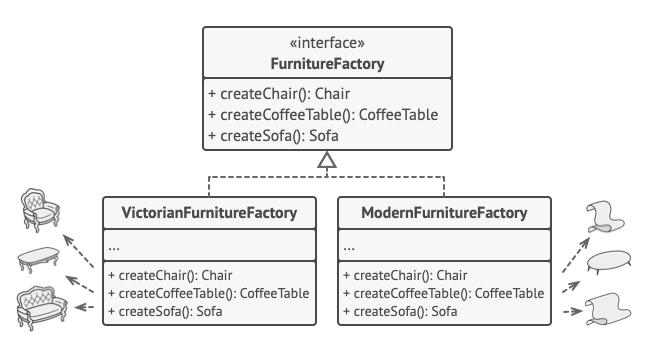
\includegraphics[width=5cm]{./Imagenes/3} 
		\end{center}
		
		\item \textbf{El constructor:} bstrae el proceso de creación de un objeto complejo, centralizando dicho proceso en un único punto.
		\begin{center}
			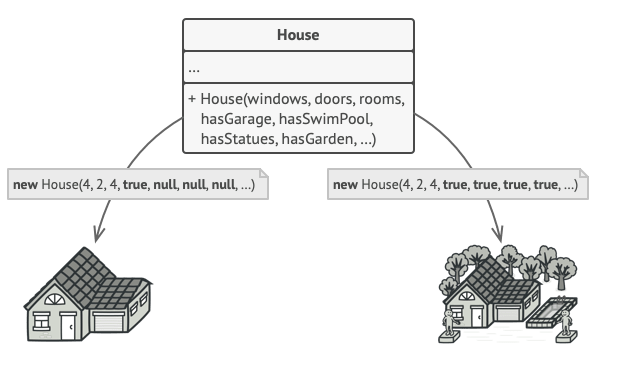
\includegraphics[width=5cm]{./Imagenes/4} 
		\end{center}
		
		\item \textbf{Método de fabricación:} crea una instancia de varias clases derivadas.
		\begin{center}
			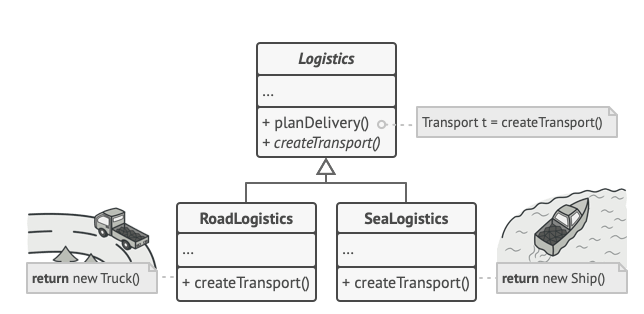
\includegraphics[width=5cm]{./Imagenes/2} 
		\end{center}
		
		\item \textbf{Grupo de objetos:}	evita la adquisición costosa y la liberación de recursos al reciclar objetos que ya no están en uso.
		\item \textbf{Prototipo:} una instancia completamente inicializada para ser copiada o clonada.
		\begin{center}
			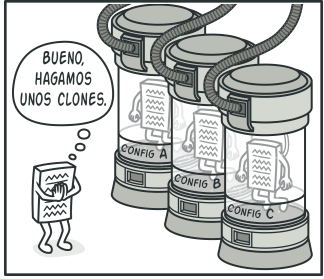
\includegraphics[width=5cm]{./Imagenes/5} 
		\end{center}
		
		\item \textbf{Instancia única:} garantiza la existencia de una única instancia para una clase y la creación de un mecanismo de acceso global a dicha instancia. Restringe la instanciación de una clase o valor de un tipo a un solo objeto.
		\begin{center}
			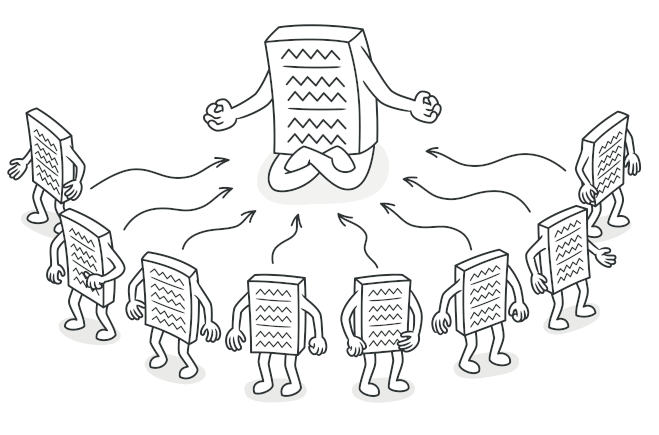
\includegraphics[width=5cm]{./Imagenes/6} 
		\end{center}
		
	\end{itemize}
	
	\item \textbf{Patrones de diseño estructural}
	\\
	\\Estos patrones de diseño tienen que ver con la composición de clases y objetos. Los patrones estructurales de creación de clases utilizan la herencia para componer interfaces. Los patrones de objetos estructurales definen formas de componer objetos para obtener una nueva funcionalidad.\cite{r}
	\begin{itemize}
		\item \textbf{Adaptador:}	crea una instancia de varias familias de clases.
			\begin{center}
			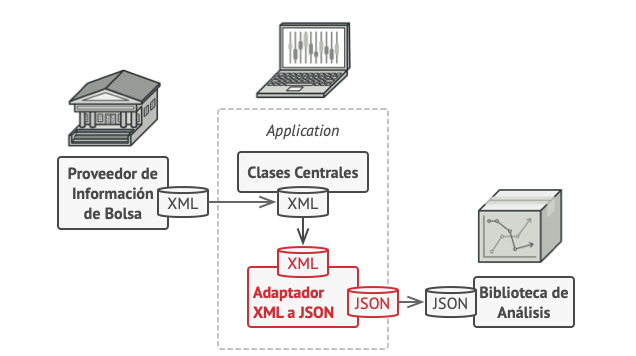
\includegraphics[width=5cm]{./Imagenes/7} 
		\end{center}
		\item \textbf{Puente:} separa la interfaz de un objeto de su implementación.
		\begin{center}
			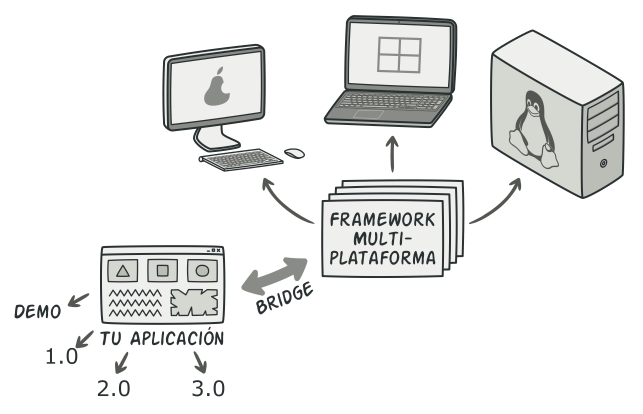
\includegraphics[width=5cm]{./Imagenes/8} 
		\end{center}
		\item \textbf{Objeto Compuesto:} permite tratar objetos compuestos como si de uno simple se tratase.
			\begin{center}
			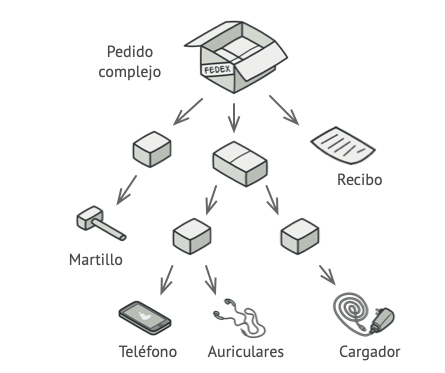
\includegraphics[width=5cm]{./Imagenes/9} 
		\end{center}
		\item \textbf{Decorador:}	permite tratar objetos compuestos como si de uno simple se tratase.
			\begin{center}
			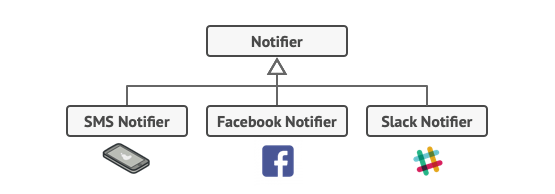
\includegraphics[width=5cm]{./Imagenes/10} 
		\end{center}
		\item \textbf{Fachada:} una sola clase que representa un subsistema completo.
			\begin{center}
			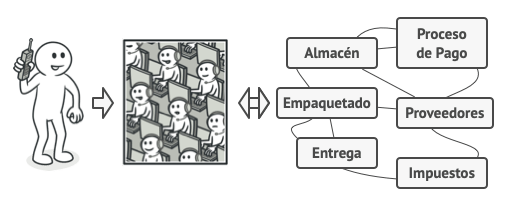
\includegraphics[width=5cm]{./Imagenes/11} 
		\end{center}
		\item \textbf{Peso ligero:} reduce la redundancia cuando gran cantidad de objetos poseen idéntica información.
			\begin{center}
			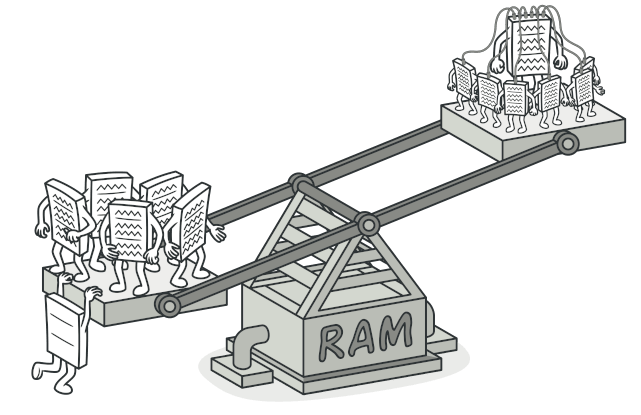
\includegraphics[width=5cm]{./Imagenes/12} 
		\end{center}
		\item \textbf{Proxy:} proporciona un intermediario de un objeto para controlar su acceso.
			\begin{center}
			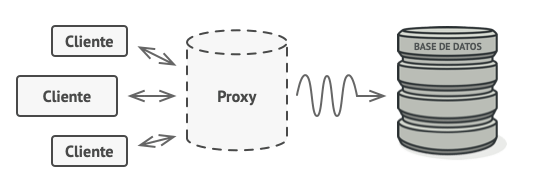
\includegraphics[width=5cm]{./Imagenes/13} 
		\end{center}
		\item \textbf{Módulo:} agrupa varios elementos relacionados, como clases, singletons, y métodos, utilizados globalmente, en una entidad única.
	\end{itemize}
	
	\item \textbf{Patrones de diseño de comportamiento}
	\\
	\\Estos patrones de diseño tienen que ver con la comunicación de objetos de Class. Los patrones de comportamiento son aquellos que se ocupan más específicamente de la comunicación entre objetos.\cite{r}
	\begin{itemize}
		\item \textbf{Cadena de responsabilidad:} permite establecer la línea que deben llevar los mensajes para que los objetos realicen la tarea indicada.
		\item \textbf{Orden:} encapsula una operación en un objeto, permitiendo ejecutar dicha operación sin necesidad de conocer el contenido de la misma.
		\item \textbf{Intérprete:} dado un lenguaje, define una gramática para dicho lenguaje, así como las herramientas necesarias para interpretarlo.
		\item \textbf{Iterador:} permite realizar recorridos sobre objetos compuestos independientemente de la implementación de estos.
		\item \textbf{Mediador:} define un objeto que coordine la comunicación entre objetos de distintas clases, pero que funcionan como un conjunto.
		\item \textbf{Recuerdo:} permite volver a estados anteriores del sistema.
		\item \textbf{Observador:} define una dependencia de uno-a-muchos entre objetos, de forma que cuando un objeto cambie de estado se notifique y actualicen automáticamente todos los objetos que dependen de él.
		\item \textbf{Estado:} permite que un objeto modifique su comportamiento cada vez que cambie su estado interno.
		\item \textbf{Estrategia:} permite disponer de varios métodos para resolver un problema y elegir cuál utilizar en tiempo de ejecución.
		\item \textbf{Método plantilla:} define en una operación el esqueleto de un algoritmo, delegando en las subclases algunos de sus pasos, esto permite que las subclases redefinan ciertos pasos de un algoritmo sin cambiar su estructura.
		\item \textbf{Visitante:} permite definir nuevas operaciones sobre una jerarquía de clases sin modificar las clases sobre las que opera.
	\end{itemize}
\end{itemize}
\subsection{Ventajas del uso de patrones}

\begin{itemize}
	\item Conforman un amplio catálogo de problemas y soluciones.
	\item Estandarizan la resolución de determinados problemas.
	\item Condensan y simplifican el aprendizaje de las buenas prácticas.
	\item Proporcionan un vocabulario común entre desarrolladores.
	
\end{itemize}

\section{Objetivos}

\begin{itemize}
\item  Los patrones son soluciones típicas a problemas comunes en el diseño orientado a objetos. Cuando una solución se repite una y otra vez en varios proyectos, alguien finalmente le pone un nombre y describe la solución en detalle. .
\item El concepto de patrones de diseño e la programación
patrones que resuelven varios problemas de diseño orientado a objetos.
\end{itemize}
\section{Ejemplo de Codigos}
\begin{center}
	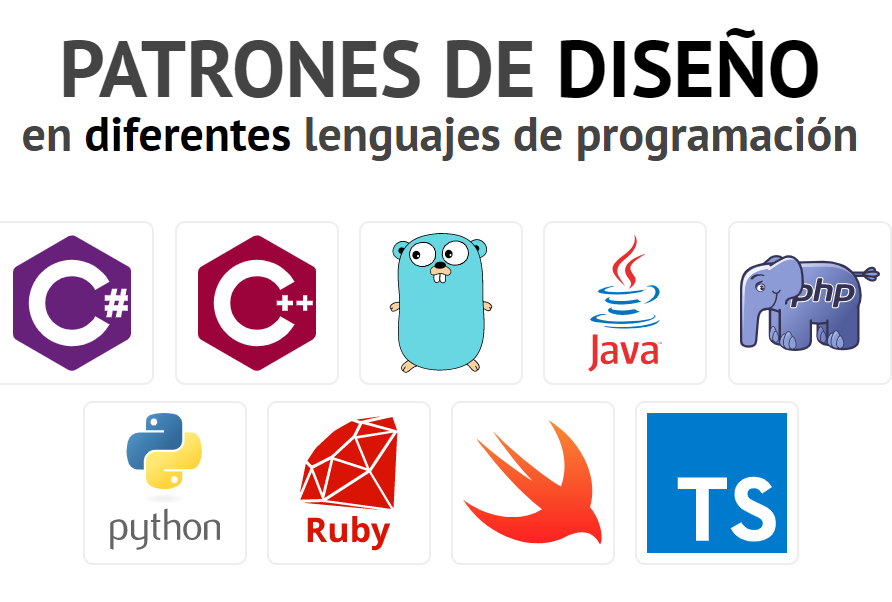
\includegraphics[width=5cm]{./Imagenes/1} 
\end{center}



%------------------------------------------------
%-----------------------------------------------------------------
\section{Conclusiones}\label{sec:6}
\begin{itemize}
	\item Los patrones de diseño ayudan al arquitecto a resolver problemas frecuentes en términos de composiciones utilizadas como esquemas de trabajo, cuyo punto de partida es un conjunto predefinido de componentes y conexiones válidas.
\end{itemize}
\section{Recomendaciones}\label{sec:7}

% Bibliografia.
%-----------------------------------------------------------------

\bibliographystyle{plain}
\bibliography{bibliografia}
https://refactoring.guru/design-patterns
http://siul02.si.ehu.es/~alfredo/iso/06Patrones.pdf
http://dominiotic.com/patrones-de-diseno/
\end{document}
